\section{Results and Analysis}
	Using the test setup and cases shown above, we were able to get the following insights.
	\subsection{DSSS}
		\subsubsection{Performance in presence of narrowband and wideband interference}~\\
			Figure \ref{fig:dsss_narrowband} shows error rate of DSSS under narrowband noise. We observe that higher \emph{chipping rates} - so broad spreading - are more robustness.
			This is due to the narrowband interference getting despread more strongly when employing higher chipping rates.
			The \emph{chip sequence length} has a small influence, which also matches the expectations. The power spectrum does not change with different chip length.
			
			Figure \ref{fig:dsss_wideband} illustrates behaviour under wideband noise, which is nearly identical for all our different testing parameters.
			We expected low \emph{chipping rates} to have better performance. The more narrow frequency spectrum should lead to higher peak power. 
			But the wideband noise is not correlated with the sent signal and the despreading does not affect it and its power spectrum.
			
			Due to our testing setup and methodology, direct comparison between the two scenarios is tedious.
			Our jammer puts out a constant overall power and so the SNRs tend to be very different when spreading more.
			We have chosen to treat narrowband and wideband noise as separate cases.
			The comparison is done in a separate test case, where we visually match the signal and noise spectra of the scenarios outlined in \cite{ISS}.
			The results of that test are shown in Figure \ref{fig:dsss_bandwidth} and discussed in the next section.
				\begin{figure}[H]
					\centering
				    \begin{subfigure}[b]{0.5\textwidth}
						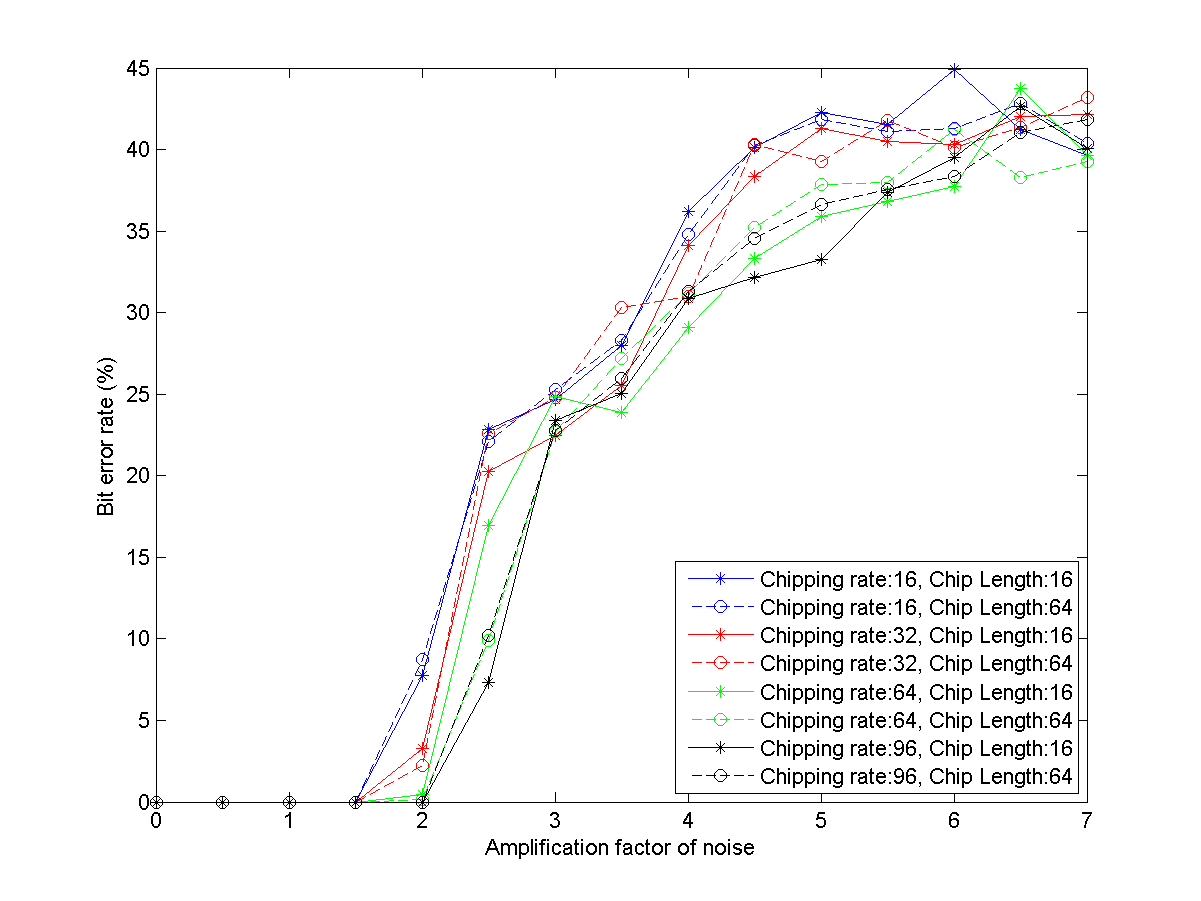
\includegraphics[width=\textwidth]{imgs/results/plot_mode_dsss-test_narrowband-rep_20-dataRate_8-dataLength_128.png}
						\caption{Narrowband noise - 8 Hz}
						\label{fig:dsss_narrowband}
					\end{subfigure}%
					~
					\begin{subfigure}[b]{0.5\textwidth}
						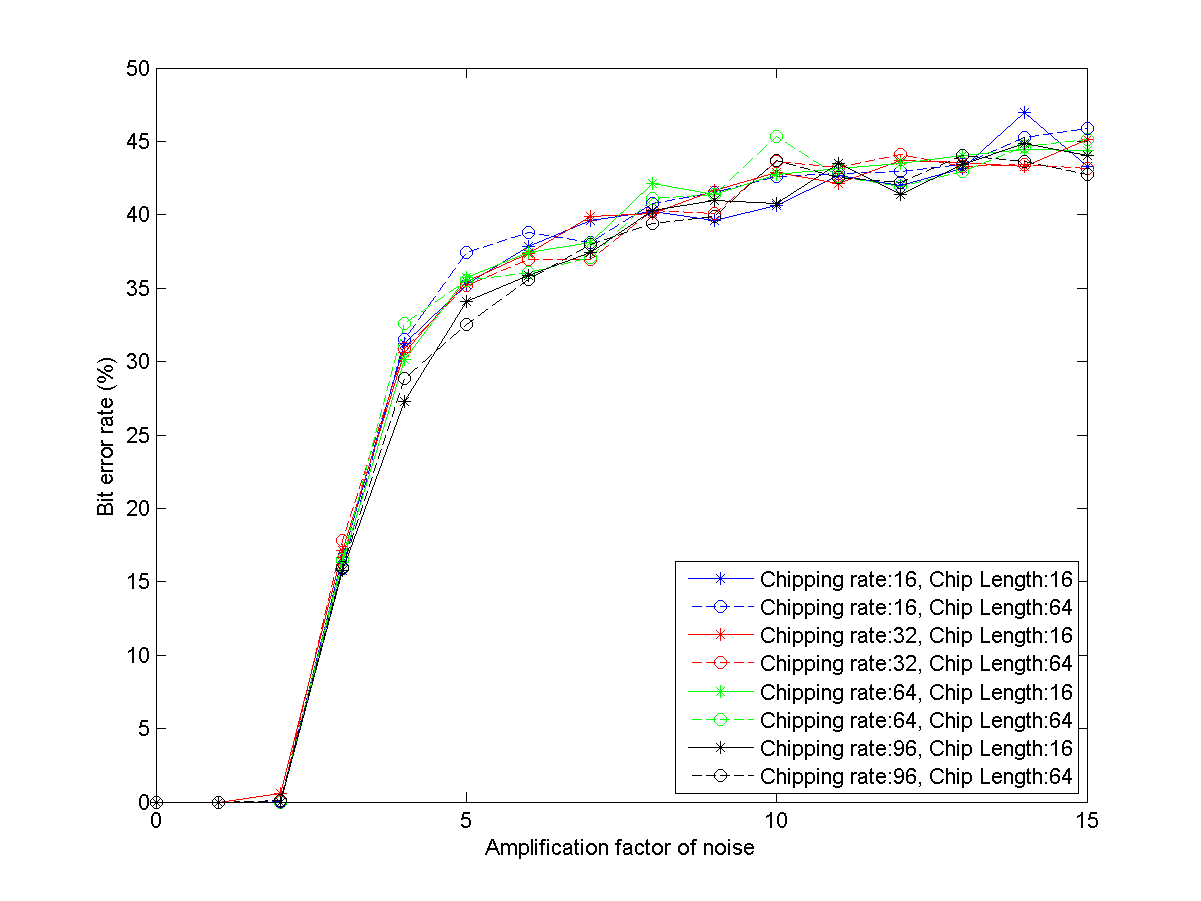
\includegraphics[width=\textwidth]{imgs/results/plot_mode_dsss-test_wideband-rep_20-dataRate_8-dataLength_128.png}
						\caption{Wideband noise - 200 Hz}
						\label{fig:dsss_wideband}
					\end{subfigure}
				\end{figure}
				
		
		\subsubsection{Performance with varying interference bandwidth and white Gaussian noise}~\\
			In Figure \ref{fig:dsss_bandwidth}, shows the results of the aforementioned test case.
			\emph{Wideband noise} has a bigger impact than \emph{narrowband noise} and high \emph{chipping rates} showing better performance than low ones.
			Since we struggled to find reliable reference values for such scenarios, the results shown should be seen as a qualitative estimation of real-world performance of DSSS and not as exact values. 
			
			Figure \ref{fig:dsss_gaussian} outlines performance of our DSSS implementation with varying levels of white Gaussian noise.
			The performance deteriorates with more added noise.
			Unexpectedly, performance was worse with low chipping rates.
			We suspect this may be due to the way MATLAB measures the SNR when using the \emph{awgn} function.
			
			\begin{figure}[H]
				\centering
				\begin{subfigure}[b]{0.5\textwidth}
					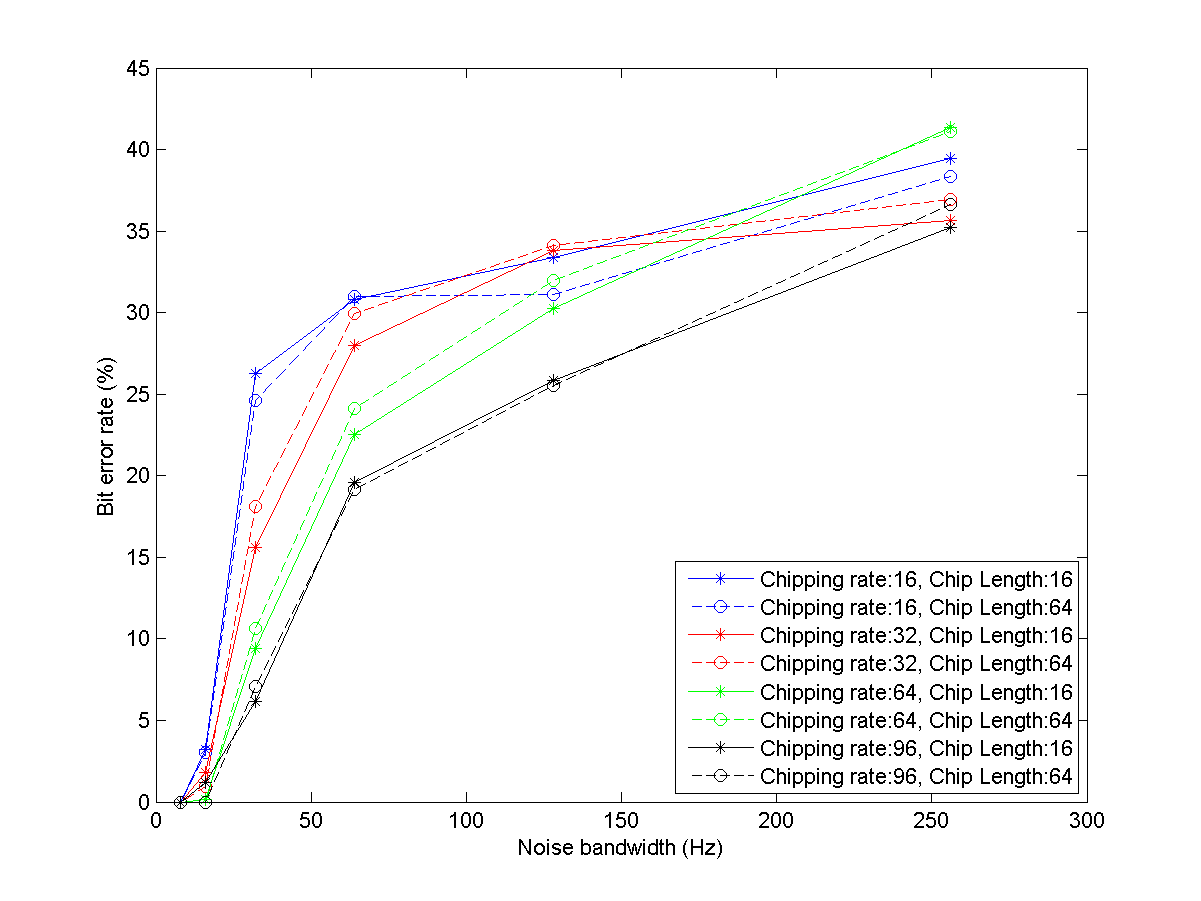
\includegraphics[width=\textwidth]{imgs/results/plot_mode_dsss-test_bandwidthAndPower-rep_20-dataRate_8-dataLength_128.png}
					\caption{Various noise bandwidths and powers}
					\label{fig:dsss_bandwidth}
				\end{subfigure}%
				~
				\begin{subfigure}[b]{0.5\textwidth}
					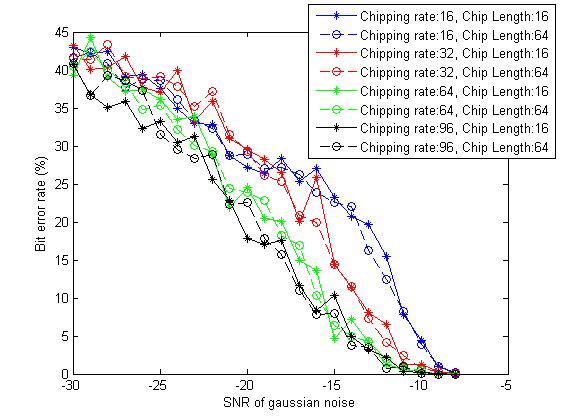
\includegraphics[width=\textwidth]{imgs/results/plot_mode_dsss-test_gaussianSNR-rep_20-dataRate_8-dataLength_128_fixedlegend.png}
					\caption{Various SNR of white Gaussian noise}
					\label{fig:dsss_gaussian}
				\end{subfigure}
			\end{figure}		
				
		\subsubsection{Performance with multiple users}~\\
				
			In Figure \ref{fig:dsss_multiuser} we see that low \emph{chipping rates} work considerably worse than high chipping rates, as the signal is spread less.
			This matches the expected behaviour.
				
			\begin{figure}[H]
				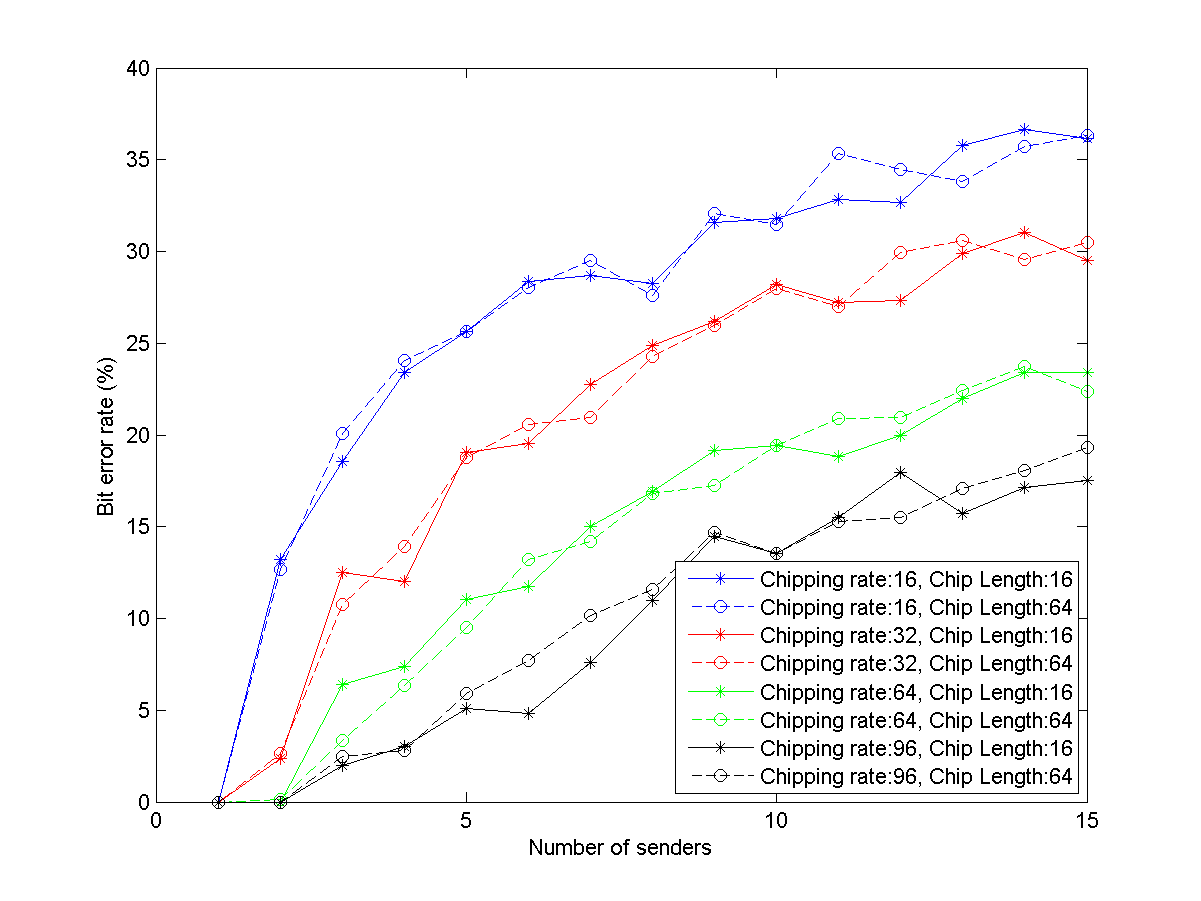
\includegraphics[width=0.5\textwidth]{imgs/results/plot_mode_dsss-test_numSenders-rep_20-dataRate_8-dataLength_128.png}
				\caption{Multiuser}
				\label{fig:dsss_multiuser}
			\end{figure}
	
	\subsection{FHSS}
		
		Before going into the exact test cases, it is important to note that there is a problem with our implementation of fast frequency hopping, as it works badly with BPSK modulation. Various websites such as \cite{web-nl} emphasize the difficulty of using coherent data detection and that FSK is most often used. However, we followed our requirements and implemented BPSK.
		
		\subsubsection{Performance in presence of narrowband and wideband interference}~\\
			The results widely match expected behaviour, with performance deteriorating the more channels are jammed and wideband noise affecting all channels - and thus all configurations - equally.
			We were not able to create configurations where without crosstalk between the different channels, so this has influenced all results.
			
			\begin{figure}[H]
				\centering
				\begin{subfigure}[b]{0.5\textwidth}
					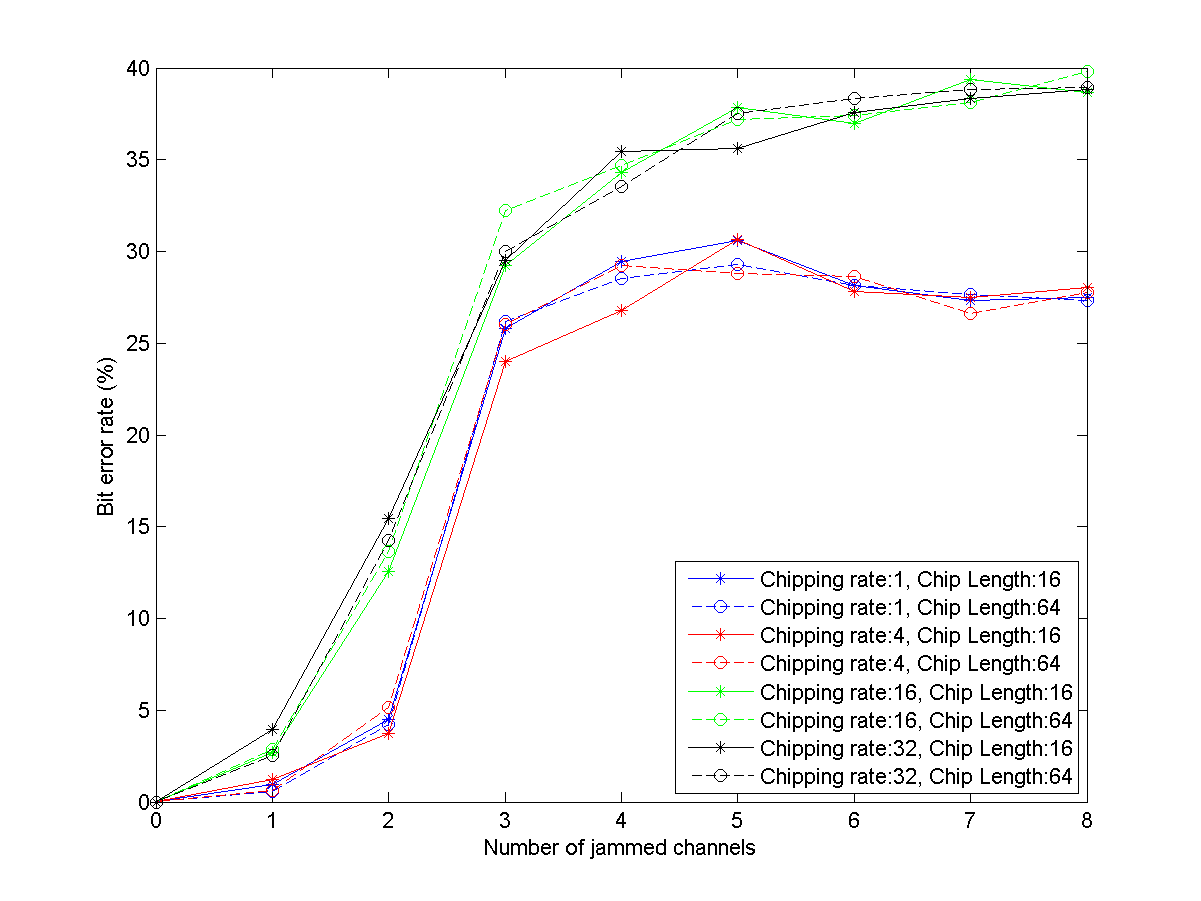
\includegraphics[width=\textwidth]{imgs/results/plot_mode_fhss-test_narrowband-rep_20-dataRate_8-dataLength_128.png}
					\caption{Narrowband noise - 64 Hz}
					\label{fig:fhss_narrowband}
				\end{subfigure}%
				~
				\begin{subfigure}[b]{0.5\textwidth}
					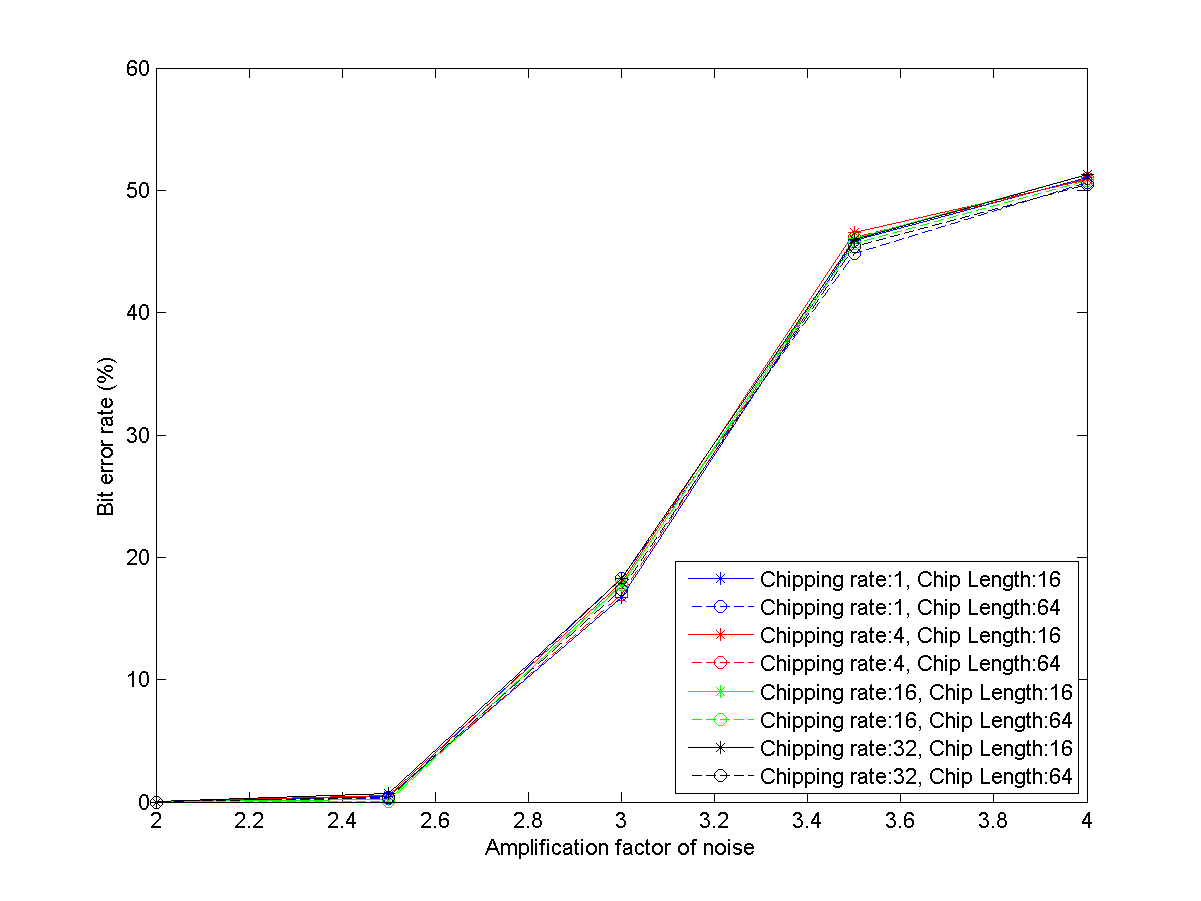
\includegraphics[width=\textwidth]{imgs/results/plot_mode_fhss-test_wideband-rep_20-dataRate_8-dataLength_128.png}
					\caption{Wideband noise - 1000 Hz}
					\label{fig:fhss_wideband}
				\end{subfigure}
			\end{figure}
			
			
		\subsubsection{Performance with varying interference bandwidth and white Gaussian noise}~\\
			The results shown in Figure \ref{fig:fhss_bandwidth} represent an estimation of performance under different noise configurations.
			The results are similar to the ones from DSSS, with better performance under the influence of narrowband interference.
			Figure \ref{fig:fhss_gaussian} shows a more streamlined result than DSSS, which is caused by the bandwidths and channel configurations being invariable under the different parameter configurations.
	
			\begin{figure}[H]
				\centering
				\begin{subfigure}[b]{0.5\textwidth}
					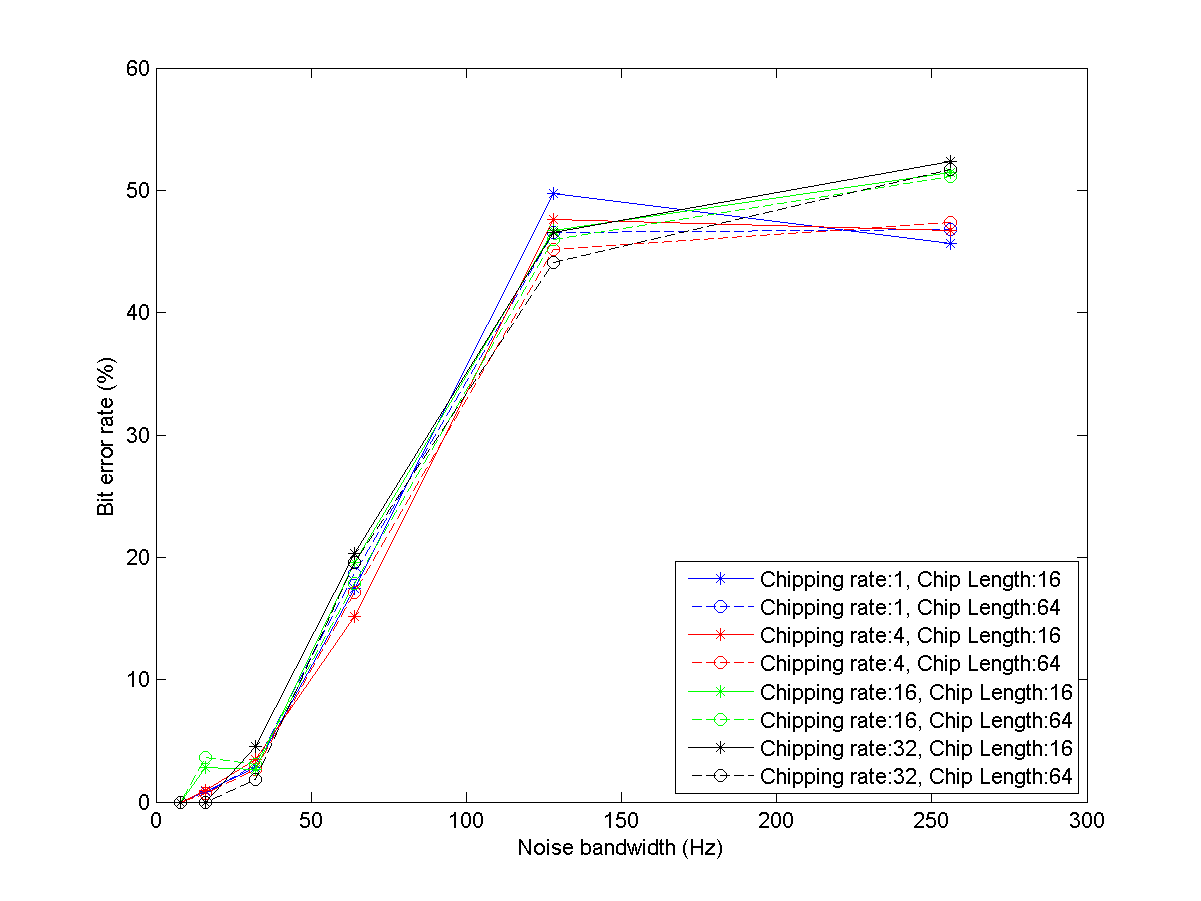
\includegraphics[width=\textwidth]{imgs/results/plot_mode_fhss-test_bandwidthAndPower-rep_20-dataRate_8-dataLength_128.png}
					\caption{Various noise bandwidth and power}
					\label{fig:fhss_bandwidth}
				\end{subfigure}%
				~
				\begin{subfigure}[b]{0.5\textwidth}
					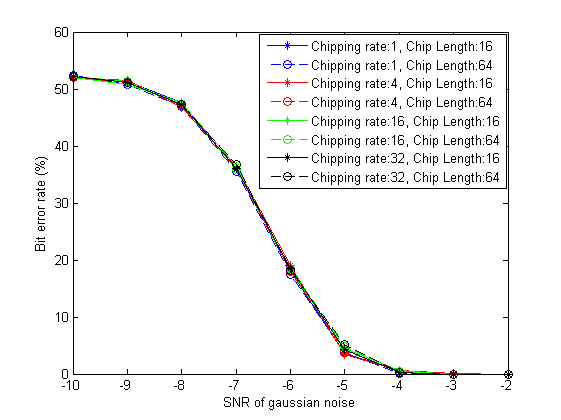
\includegraphics[width=\textwidth]{imgs/results/plot_mode_fhss-test_gaussianSNR-rep_20-dataRate_8-dataLength_128_fixedlegend.png}
					\caption{Various SNR of white Gaussian Noise}
					\label{fig:fhss_gaussian}
				\end{subfigure}
			\end{figure}
		
		\subsubsection{Performance with multiple users}~\\
			The results shown match the expected behaviour. The performance deteriorates quickly and bottoms at 40-50 \% BER when the number of users approaches the number of channels.
			\begin{figure}[H]
				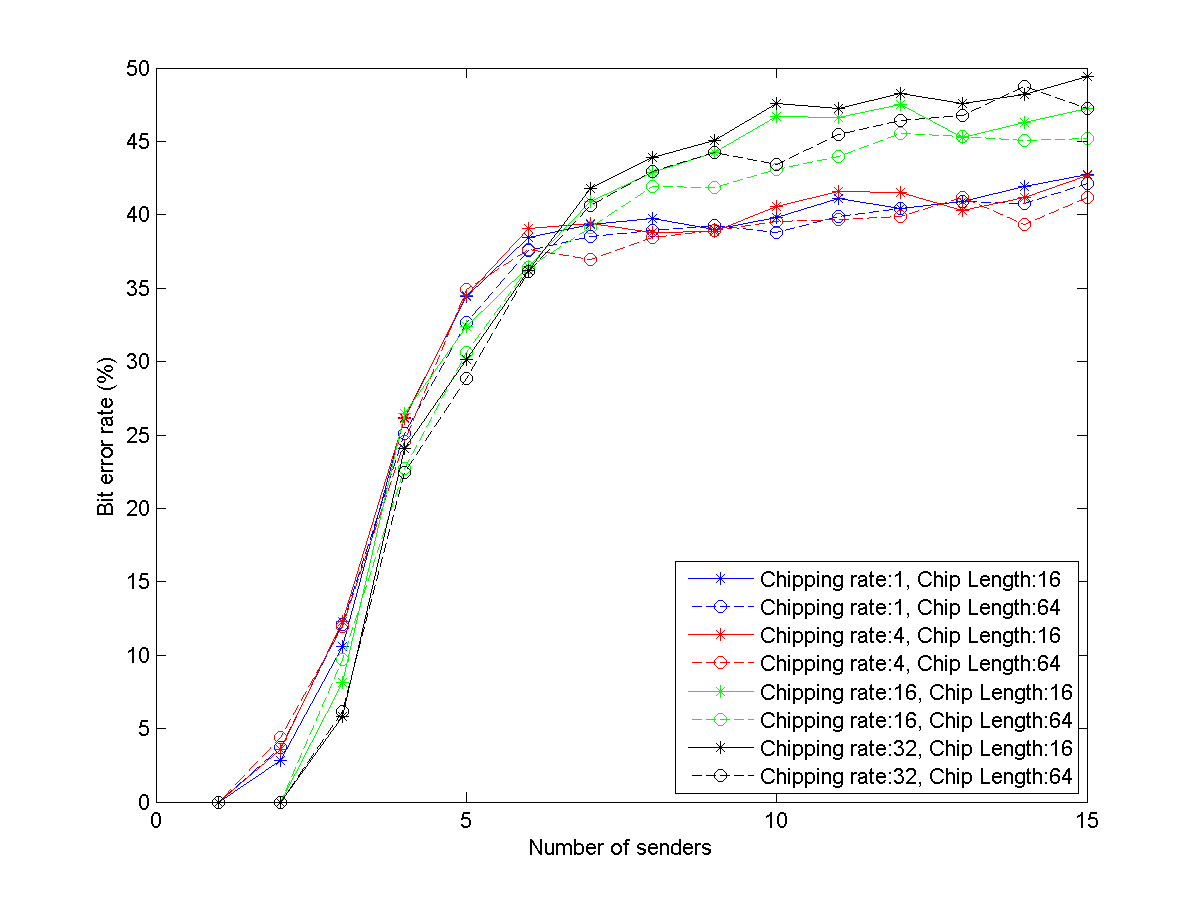
\includegraphics[width=0.5\textwidth]{imgs/results/plot_mode_fhss-test_numSenders-rep_20-dataRate_8-dataLength_128.png}
				\caption{Multiuser}
				\label{fig:fhss_multiuser}
			\end{figure}